\chapter{Résumé de thèse}
\section*{Introduction}
La tomographie par émission de positons (TEP) est passée, dans les dernières décennies, d'un outil utilisé principalement dans les applications de recherche à un outil d'imagerie clinique qui a un rôle majeur dans de nombreuses applications cliniques et applications de recherche clinique~\cite{Meikle2021}. 
En combinaison avec plusieurs radiotraceurs disponibles, qui permettent à l'imagerie TEP de cibler et de recueillir des informations sur la fonction au niveau moléculaire, la TEP peut fournir des informations uniques sur les biomarqueurs. La nature non invasive de l'imagerie TEP, combinée à son potentiel de reproductibilité entièrement quantitative et fiable des informations sur les biomarqueurs, sont des aspects très importants qui la rendent désirable dans le cadre de la médecine de précision~\cite{Subramaniam2017,Meikle2021}.
La plupart des applications cliniques actuelles de la TEP se concentrent sur l'imagerie statique et des mesures qualitatives et semi-quantitatives. Mais la TEP a la capacité de fournir des paramètres biologiquement pertinents entièrement quantitatifs, en surveillant la cinétique du traceur et le comportement dynamique avec un balayage dynamique sur une période de temps. Ces informations peuvent être utilisées pour générer des images paramétriques qui décomposent les informations en paramètres de modèles qui guident le comportement dynamique. Ceux-ci peuvent être utilisés pour identifier les différentes régions qui contribuent à un comportement différent d'absorption du traceur et peuvent être liés à des différences dans la fonction sous-jacente et la pathophysiologie, avec une applicabilité dans la recherche et les futures applications cliniques.

La majorité des scanners cliniques offrent un champ de vision axial (Axial Field of View; A-FOV) limité, entre 15 et 26 cm~\cite{Vandenberghe2020}. En imagerie statique, la couverture du corps entier est obtenue en combinant plusieurs positions du lit à différents emplacements axiaux pour étendre le champ de vision effectif~\cite{Schubert1996}, ou par un mouvement axial continu du lit (Continuous Bed Movement; CBM)~\cite{Panin2014}.
De même, pour réaliser une imagerie dynamique sur l'ensemble du corps, des protocoles dynamique du corps entier (Dynamic Whole Body; DWB) ont été développés, qui utilisent de multiples passages répétés sur le corps entier~\cite{Karakatsanis2011,Karakatsanis2013,Rahmim2019}. 
Mais ces protocoles d'acquisition posent des défis qui proviennent des lacunes temporelles résultantes dans les données dynamiques acquises de toute position de lit donnée. Ces écarts sont introduits à chaque position du lit par le temps consacré à l'imagerie d'autres positions du lit et par les retards du système de scanner dus au temps nécessaire pour déplacer le lit dans la direction axiale et préparer l'acquisition de la position suivante du lit. Mais cette acquisition résulte en une forte réduction à la fois des nombre de détections totaux collectés pour chaque position lit et de la fréquence d'échantillonnage temporel. En outre, l'acquisition d'informations sur les changements temporels rapides dans la phase initiale de l'étude dynamique est compromise, car ces changements ne sont pas échantillonnés de manière adéquate pour toutes les positions du lit. Par conséquent, les estimations des paramètres à partir d'acquisitions TEP dynamiques du corps entier sont potentiellement compromises par les limitations ci-dessus dans leur précision et leur exactitude.
La génération d'images paramétriques à partir de données dynamiques nécessite l'ajustement du modèle dynamique d'intérêt sur les courbes d'activité temporelle (Time activity curve; TAC) pour chaque voxel de l'image. En raison de la mauvaise statistique et du bruit élevé associés aux mesures de TAC au niveau du voxel, qui sont encore dégradés par les protocoles d'acquisition DWB, les estimations d'images paramétriques peuvent être fortement erronés par le bruit et potentiellement biaisées.
L'objectif principal de cette thèse était d'explorer l'optimisation de l'acquisition et les nouvelles stratégies de reconstruction pour améliorer les cartes paramétriques du corps entier. 

Les contributions peuvent être séparées en trois parties. La première partie se concentre sur l'optimisation du protocole DWB sur un scanner clinique TEP/IRM, visant à réduire les écarts temporels des acquisitions DWB et à augmenter les comptes collectés ainsi que la fréquence d'échantillonnage. 
La deuxième partie se concentre sur l'utilisation d'algorithmes de reconstruction dynamique pour améliorer l'imagerie paramétrique de la TEP , en utilisant des données simulées et réelles.
La troisième et dernière partie est consacrée à l'application des algorithmes de reconstruction dynamique évalués sur des données réelles d'une première étude pharmacocinétique chez l'homme appelée IsotoPK~\cite{Marie2019}, afin de fournir une régularisation temporelle des cartes d'activité et de générer des cartes paramétriques pertinentes pour cette étude.
Dans cette application à des données DWB réelles, des considérations supplémentaires ont été faites pour tenir compte des erreurs de modélisation dans la reconstruction en utilisant des modèles résiduels adaptatifs dans la boucle de reconstruction.

\section*{Contributions}
\subsection*{TEP dynamique multi-lits pour le corps entier: Optimisation de l'acquisition}
Dans ce chapitre, nous examinons les résultats des performances d'acquisition d'un protocole DWB mis en œuvre sur le scanner Signa TEP/IRM dans le cadre de l'étude pharmacocinétique IsotoPK~\cite{Marie2019}, en termes de délais et d'écarts temporels qui en résultent.
Nous décrivons ensuite le développement et la mise en œuvre d'un protocole expérimental entièrement automatisé pour l'imagerie DWB qui a été conçu dans le but de réduire les délais d'acquisition et de permettre une plus grande flexibilité sur l'acquisition. Cette protocole a été conçu dans le but de réduire ces délais en automatisant entièrement le processus d'acquisition et en enregistrant en continu les informations TEP dans un seul fichier en mode liste pour toutes les positions du lit pendant toute la durée de l'étude DWB.
En utilisant une telle stratégie d'acquisition, les délais entre les positions du lit et les balayages WB ont été réduits au temps pris par le seul mouvement physique de la table du scanner. 
La performance du protocole d'acquisition expérimental nouvellement développé a été testée sur une étude de un primate non humain et les résultats ont été comparés au protocole utilisé dans l'étude IsotoPK.

En utilisant les informations temporelles des données TEP brutes IsotoPK extraites de 7 examens de sujets, les délais moyens de ce protocole DWB à 5 positions de lit ont fourni un délai intra-lit moyen de 5,69 s \mbox{(95\%CI : 5,63-5,75)} et un délai moyen entre les balayages WB de 26,17 s (95\%CI : 26,13-26,22).
 
Après des tests initiaux à l'aide de fantômes, le protocole DWB automatisé a été testé sur une étude \gls{nhp} utilisant un nouveau traceur $^{18}$F-Crizotinib. Le examen a été effectué avec l'utilisation de 3 positions de lit, pour un total de 28 passages de WB.
La figure~\ref{Resumefig3_1:Macaque_Head_Curve_Phases} montre les 260 premières secondes de la courbe de acquisition des données enregistrées en mode liste, avec les phases et les positions du lit superposées. Celles-ci montrent la phase initiale de lit unique dynamique (Dynamic Single Bed; DSB) qui a été conduite centrée sur le cerveau
pendant une durée de 90 s, suivie par les premières acquisitions de passes WB de trois positions de lit.
L'estimation des délais (écarts temporels) pour cette étude utilisant le protocole d'acquisition automatisé a été faite en utilisant les informations enregistre. Les résultats ont montré un délai moyen intra-lit de 3,77 s (95\%CI : 3,62-3,91) et un délai moyen entre les balayages de \mbox{4,6 s} (95\%CI : 4,53-4,67). 
Pour faire une comparaison entre le protocole IsotoPK de 5 positions de lit et le protocole automatisé qui a été testé en utilisant 3 positions de lit, le temps de retard entre les balayages de cette étude a été estimé en utilisant une approximation à 7,66 s.

\begin{figure} [ht!]
\centering
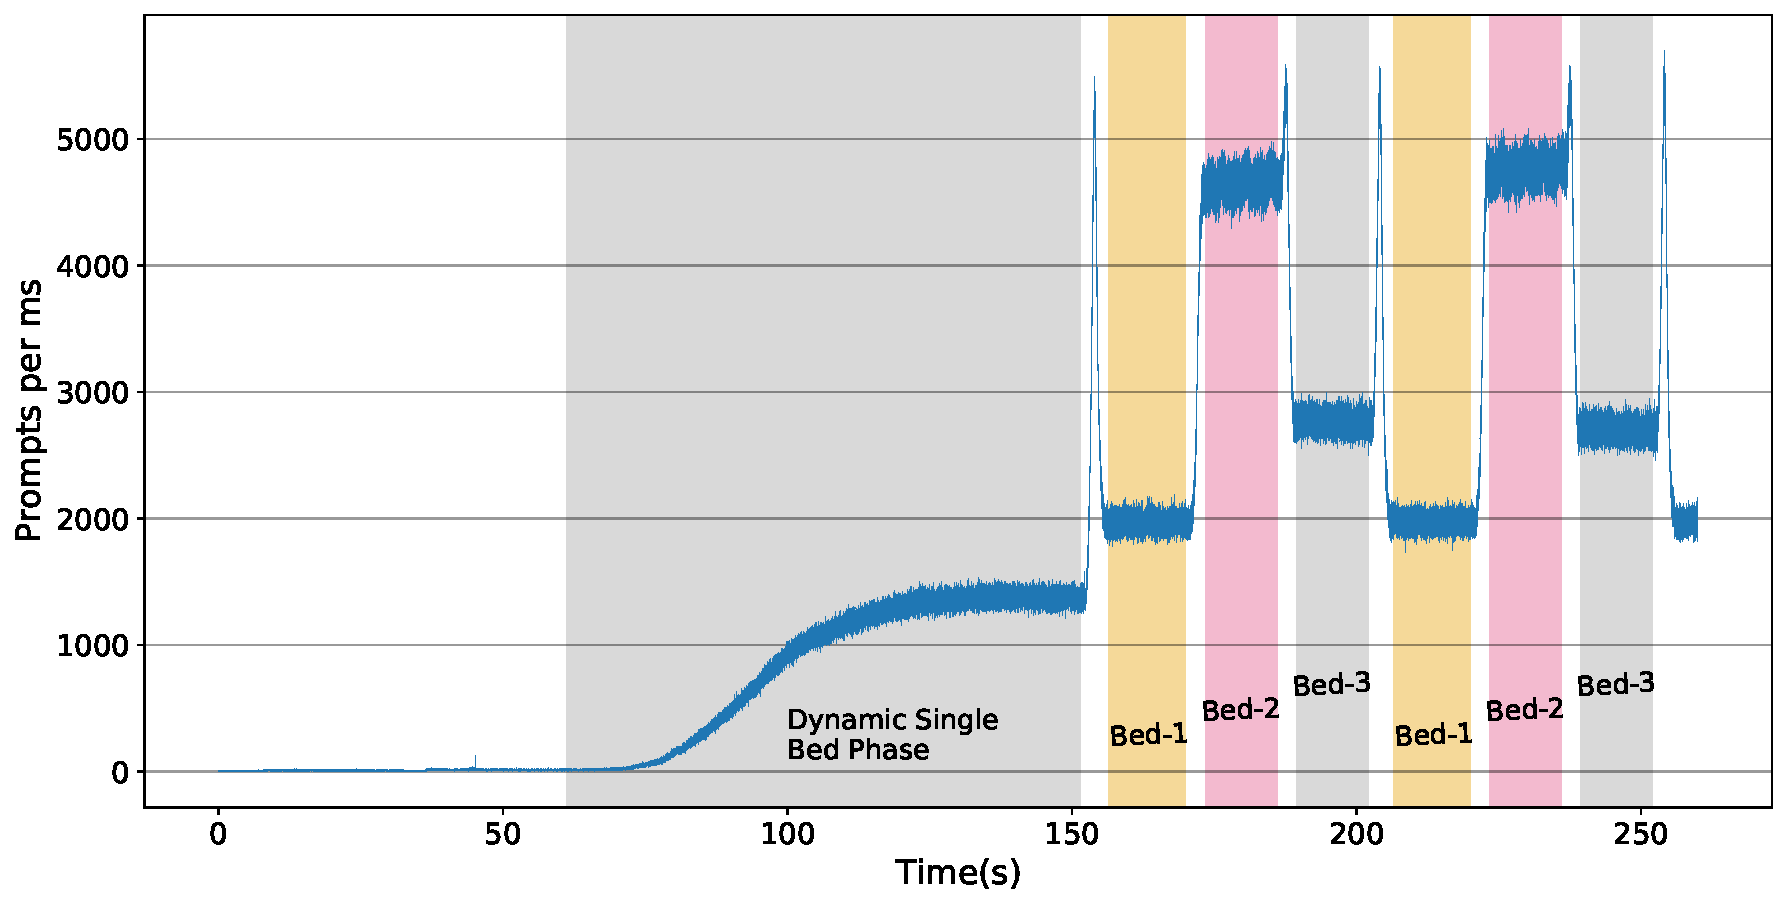
\includegraphics[scale=0.45,angle=0]{./Resume/3_1_Macaque_Head_curve_Phases.pdf}
\caption{Courbe de tête (taux de détections en fonction du temps) de l'étude du primate acquis montrant les phases DSB et DWB de l'acquisition et les trois positions du lit DWB.}
\label{Resumefig3_1:Macaque_Head_Curve_Phases}
\end{figure}

\begin{figure} [ht!]
\centering
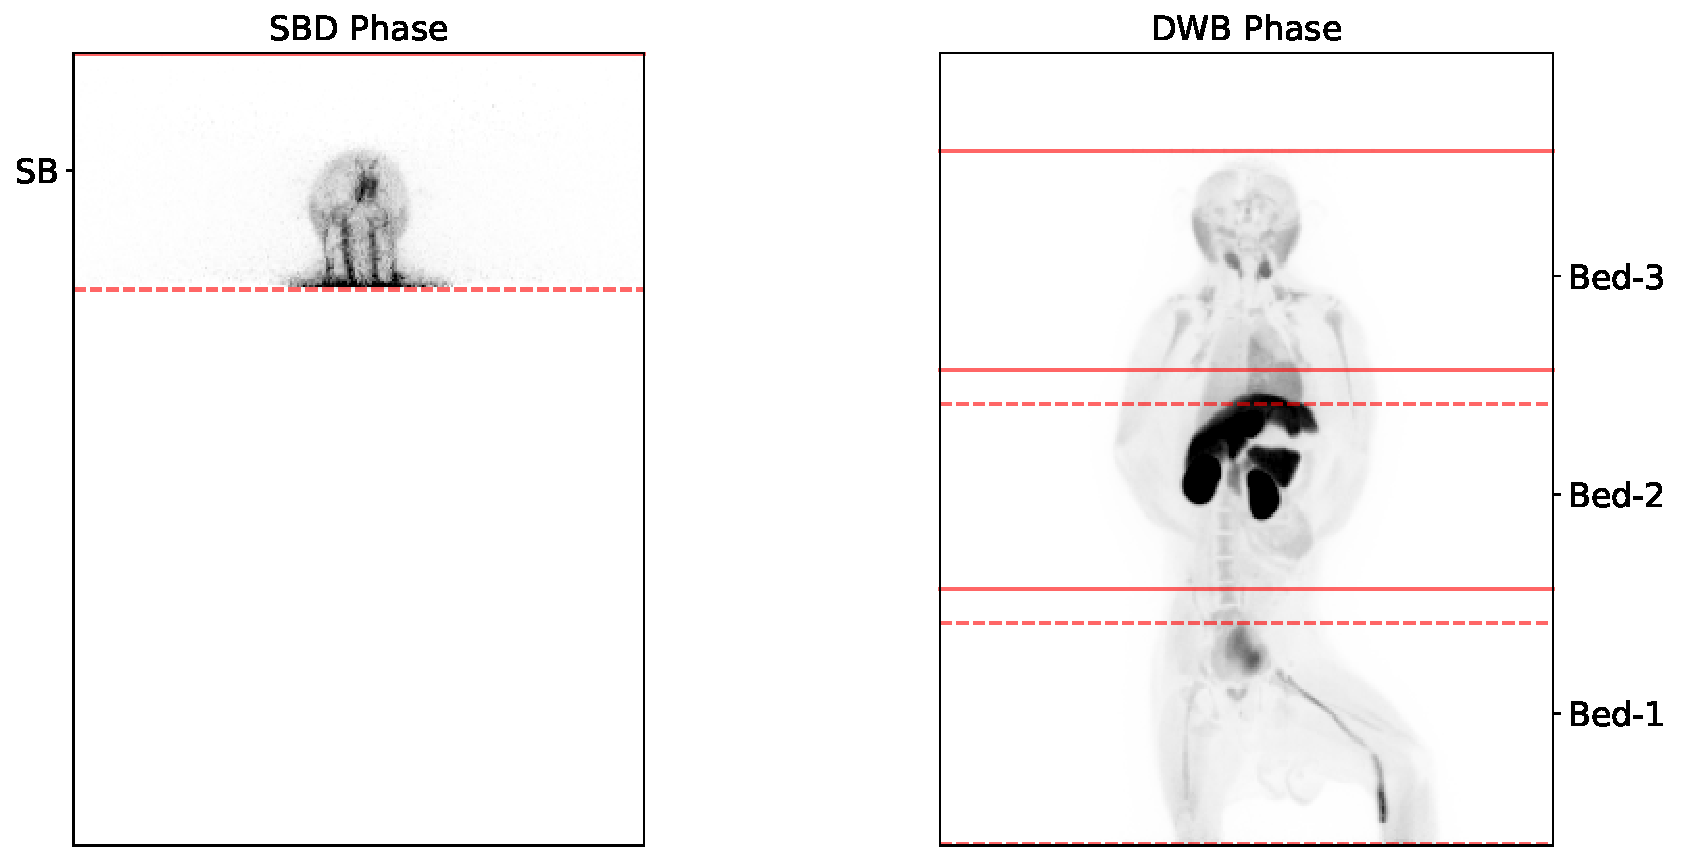
\includegraphics[scale=0.45,angle=0]{./Resume/3_1_Macaque_PET.pdf}
\caption{Vues de projection d'intensité maximale des images TEP reconstruites de l'étude primate, pour les deux phases de l'acquisition.}
\label{Resumefig3_1:Macaque_PET}
\end{figure}

L'utilisation du protocole entièrement automatisé a permis de réduire considérablement les délais, tout en simplifiant l'acquisition des ensembles de données DWB par une automatisation complète. Ces réductions des délais peuvent se traduire par une amélioration des statistiques d'acquisition ainsi que par un balayage temporel plus rapide, ce qui peut être essentiel dans les premières phases de l'acquisition du DWB. 
De considérations supplémentaires sur les vitesses de table admissibles pour la sécurité et le confort des patients doivent être faites avant d'utiliser ce protocole sur des sujets humains. 

\subsection*{Reconstruction dynamique de données DWB: Une étude de simulation}
La génération d'images paramétriques à partir de données dynamiques peut être un défi lorsqu'elle est appliquée à des données DWB.
En raison de la mauvaise statistique et du bruit élevé associés aux mesures de TAC au niveau du voxel, en particulier pour les acquisitions DWB, les estimations d'images paramétriques peuvent être fortement erronés par le bruit et potentiellement biaisées. 
L'utilisation de la reconstruction dynamique directe a été proposée pour améliorer cette tâche en utilisant des modèles dynamiques directement dans la reconstruction. Ces techniques permettent une modélisation plus précise du bruit des données TEP brutes dans le processus de reconstruction et peuvent améliorer le bruit des images paramétriques et réduire le biais~\cite{Reader2014}. 
Dans ce chapitre, nous décrivons l'implémentation d'algorithmes de reconstruction dynamique au sein de la plateforme open-source de reconstruction entièrement quantitative CASToR~\cite{Merlin2018}, qui a été réalisée dans le cadre de ce projet. Nous évaluons ensuite les performances des algorithmes de reconstruction dynamique à l'aide de simulations pour l'imagerie DWB TEP au fluorodésoxyglucose ([$^{18}$F]FDG), pour différents modèles dynamiques et pour différents protocoles d'acquisition en DWB. Les simulations ont été réalisées à l'aide du fantôme cérébral numérique Zubal~\cite{Zubal1994}. Les résultats ont finalement été démontrés dans une étude TEP dynamique réelle.
L'évaluation a porté spécifiquement sur l'imagerie paramétrique Patlak $K_i$ et l'utilisation du modèle Patlak~{Patlak1985} et de l'analyse spectrale~{Cunningham1993} pour la reconstruction dynamique. Le modèle d'analyse spectrale a été utilisé avec trois ensembles différents de nombres de fonctions de base (17, 9 et 6). Le modèle de Patlak n'est valable que pour les données après que les conditions d'état stationnaire sont atteintes ($t>t_{ss}\approx\mathrm{15 min}$), alors que le modèle spectral peut s'adapter à toutes les données dynamiques. Afin de comparer plus étroitement les deux modèles pour la reconstruction 4D, des comparaisons ont été faites en utilisant le modèle spectral avec toutes les données dynamiques ainsi qu'avec les données dynamiques après $t_{ss}$ (reconstructions marquées avec $t > t_{ss}$).

Les résultats de la comparaison entre la reconstruction dynamique (4D) et la reconstruction image par image (3D, suivie d'une modélisation cinétique post-reconstruction) ont été effectués pour deux régions du fantôme cérébral. Les comparaisons ont été effectuées en utilisant des mesures au niveau du VOI et du voxel (respectivement \%Bias vs \%CoV et \%RMS Bias vs \%RMS CoV). Ces résultats sont présentés dans la figure~\ref{Resumefig:3_2_DynamicModels}.
Les résultats montrent que la reconstruction dynamique utilisant le modèle de Patlak (4D Patlak) sur les données DWB peut fournir des résultats proches de ceux des protocoles à lit unique sans lacunes temporelles dans leurs données. En outre, la reconstruction 4D Patlak a fourni une gamme plus courte de valeurs de biais avec des itérations croissantes par rapport à la reconstruction 3D. La reconstruction dynamique avec le modèle spectral (4D Spectral) a fourni des résultats encore meilleurs que la reconstruction Patlak 4D des données DWB et la reconstruction 3D des données dynamiques à lit unique. La reconstruction spectrale 4D, utilisant 9 fonctions de base, a permis d'obtenir un compromis optimal entre une faible variance/bruit et un faible biais. La reconstruction spectrale 4D utilisant des données $t > t_{ss}$ a donné lieu à un comportement similaire en termes de variance et de bruit à celui de la reconstruction Patlak 4D, avec des caractéristiques de biais légèrement inférieures sur certaines régions par rapport à la reconstruction Patlak.

Les résultats appliqués à l'ensemble de données réelles, qui ont été répertoriées pour émuler le cadrage et les écarts d'acquisition du DWB, ont montré que le rapport contraste/bruit (CNR) le plus élevé sur une tumeur dans les poumons a été obtenu par les reconstructions 4D Spectral, suivies par la reconstruction Patlak 4D. Les deux méthodes de reconstruction dynamique ont fourni un rapport contraste/bruit plus faible que la reconstruction 3D effectuée sur des données DWB ou des données dynamiques à lit unique sans lacunes. Une évaluation du bruit paramétrique de l'image dans le foie a montré un comportement similaire pour toutes les reconstructions 4D, avec un bruit plus faible que la reconstruction 3D des mêmes données DWB mais plus élevé que la reconstruction 3D des données dynamiques à lit unique.
Les images paramétriques $K_i$ issues des reconstructions 3D et 4D des données réelles aux itérations avec des valeurs SD du foie correspondantes sont présentées dans la figure~\ref{Resumefig:RealKiMontage}. 
%
\begin{figure} [ht!]
\centering
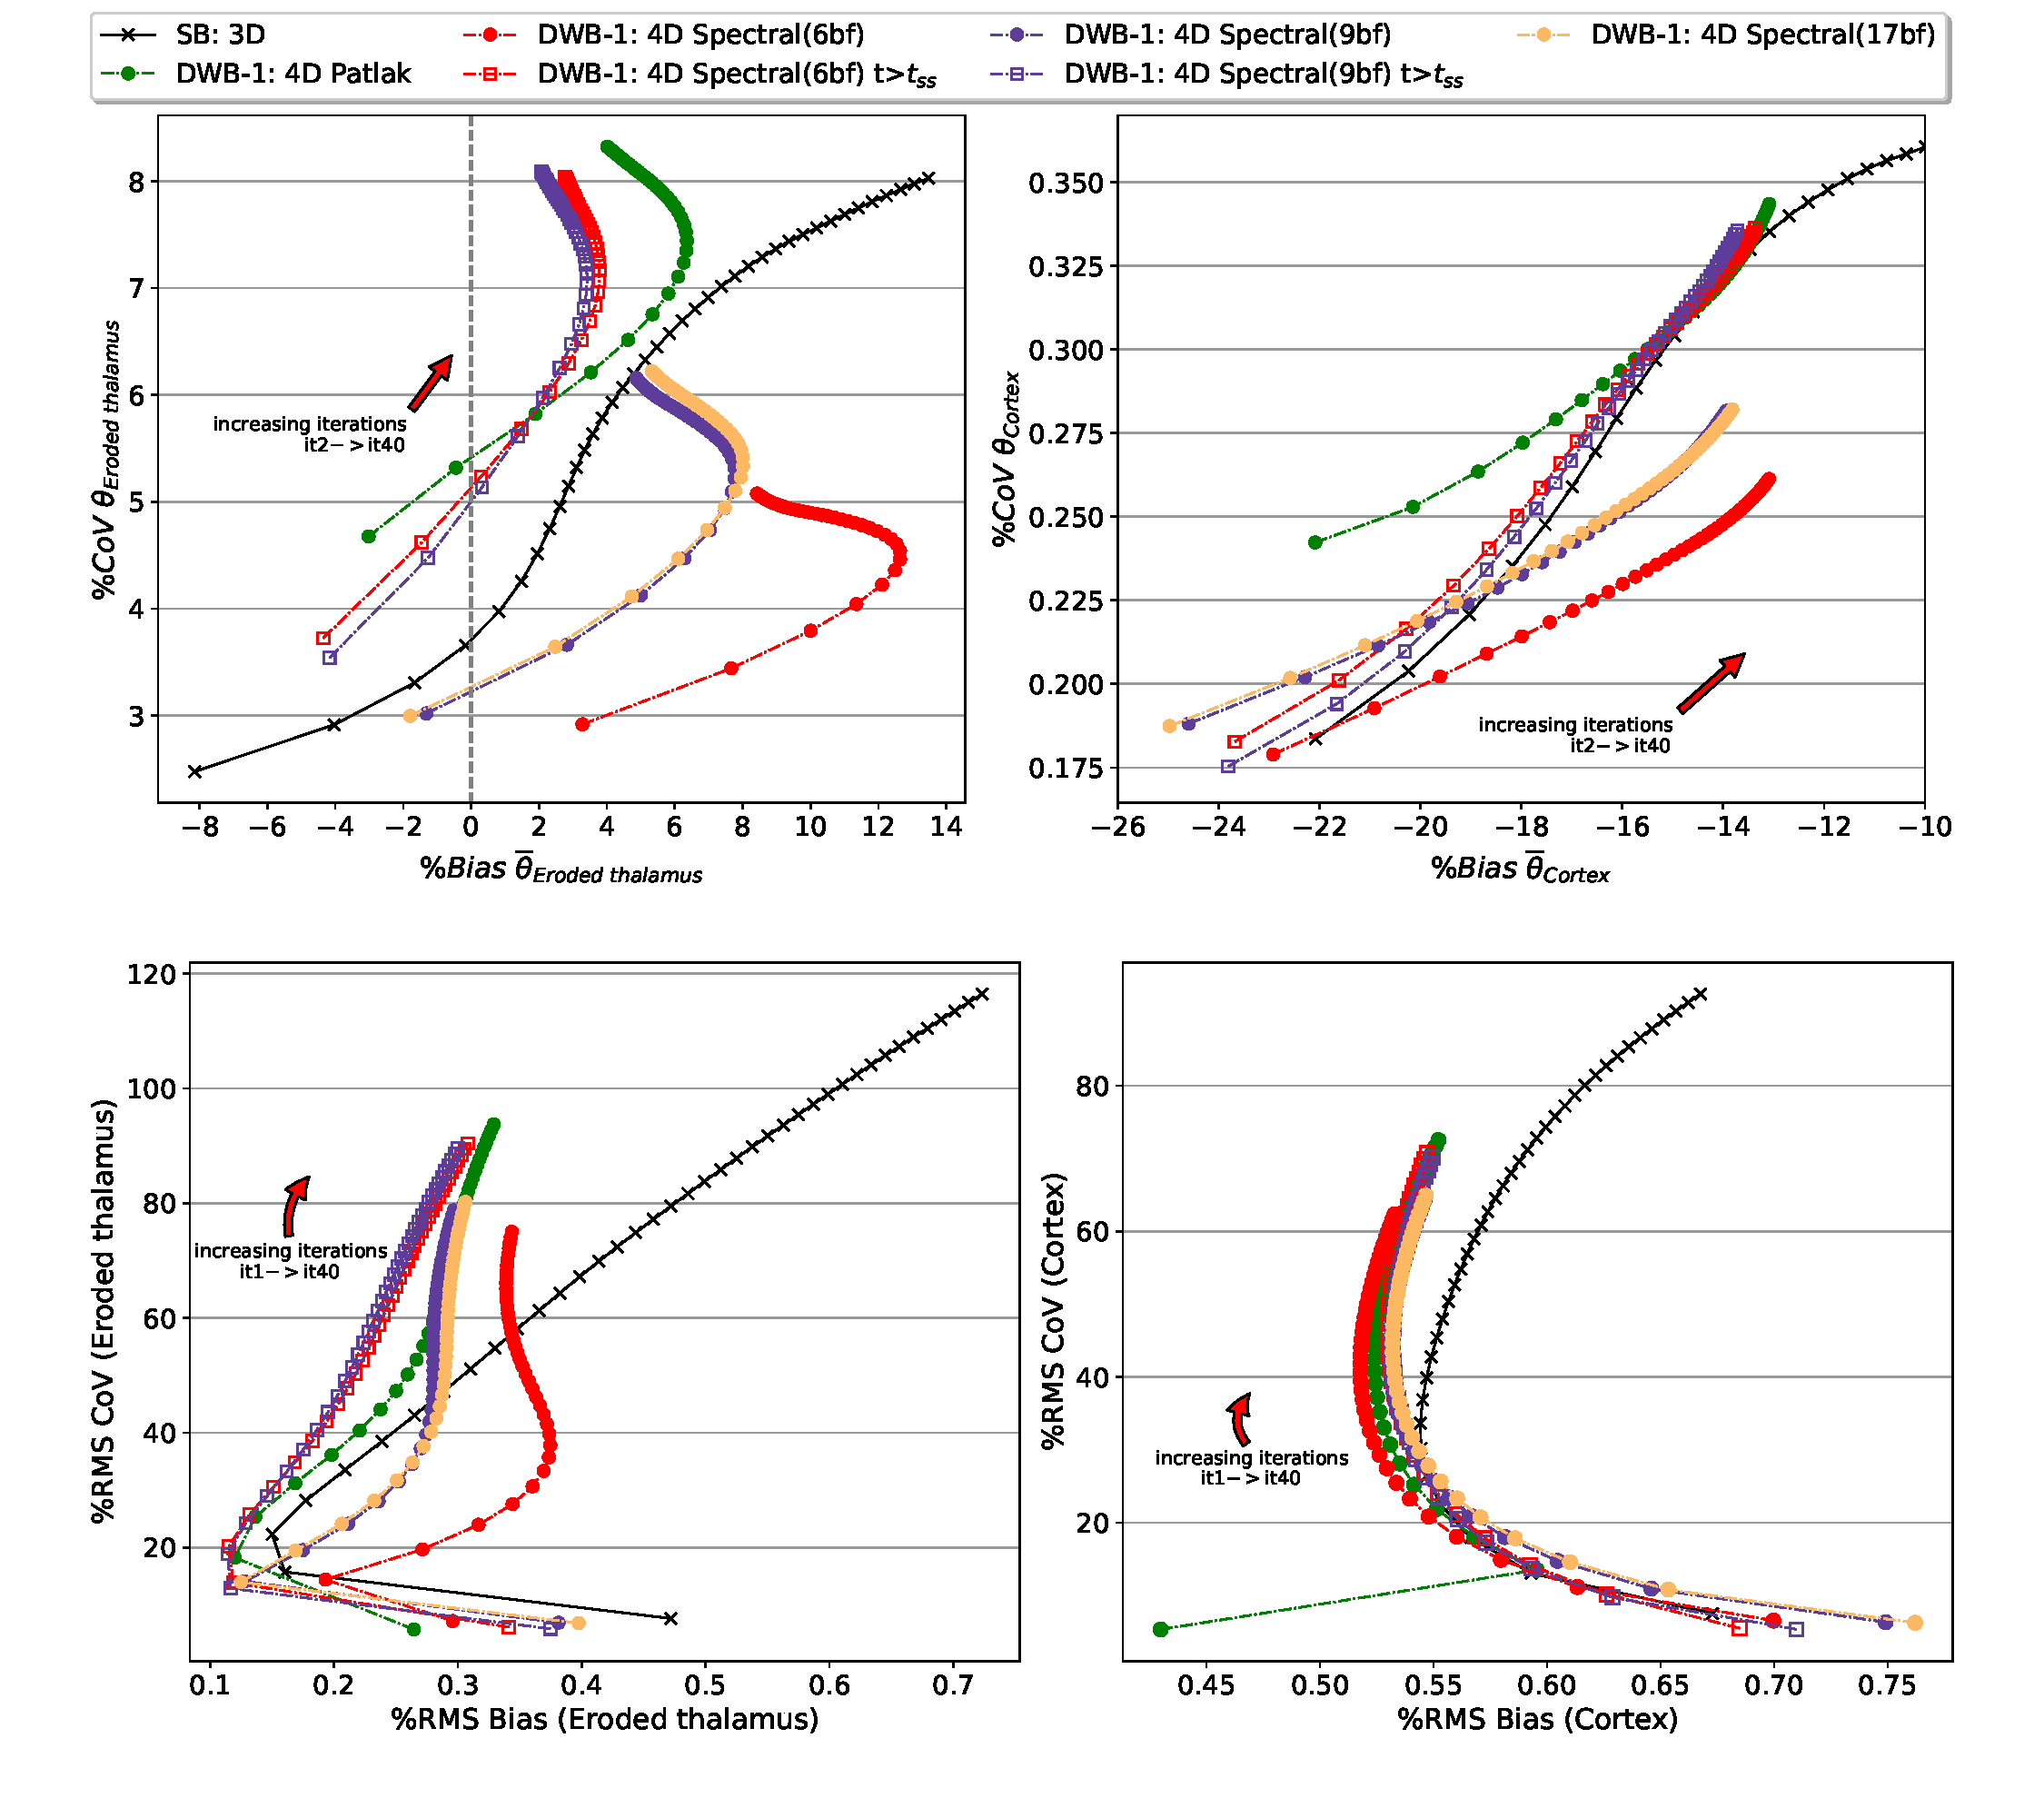
\includegraphics[scale=0.42,angle=0]{./Resume/3_2.pdf}
\caption{Simulation: Courbes de compromis entre le bruit et le biais du thalamus (gauche) et du cortex (droite) pour les reconstructions 4D des données du protocole DWB-1. Métriques basées sur les VOI (haut) et sur les voxels (bas).}
\label{Resumefig:3_2_DynamicModels}
\end{figure} 
%
\begin{figure} [ht!]
\centering
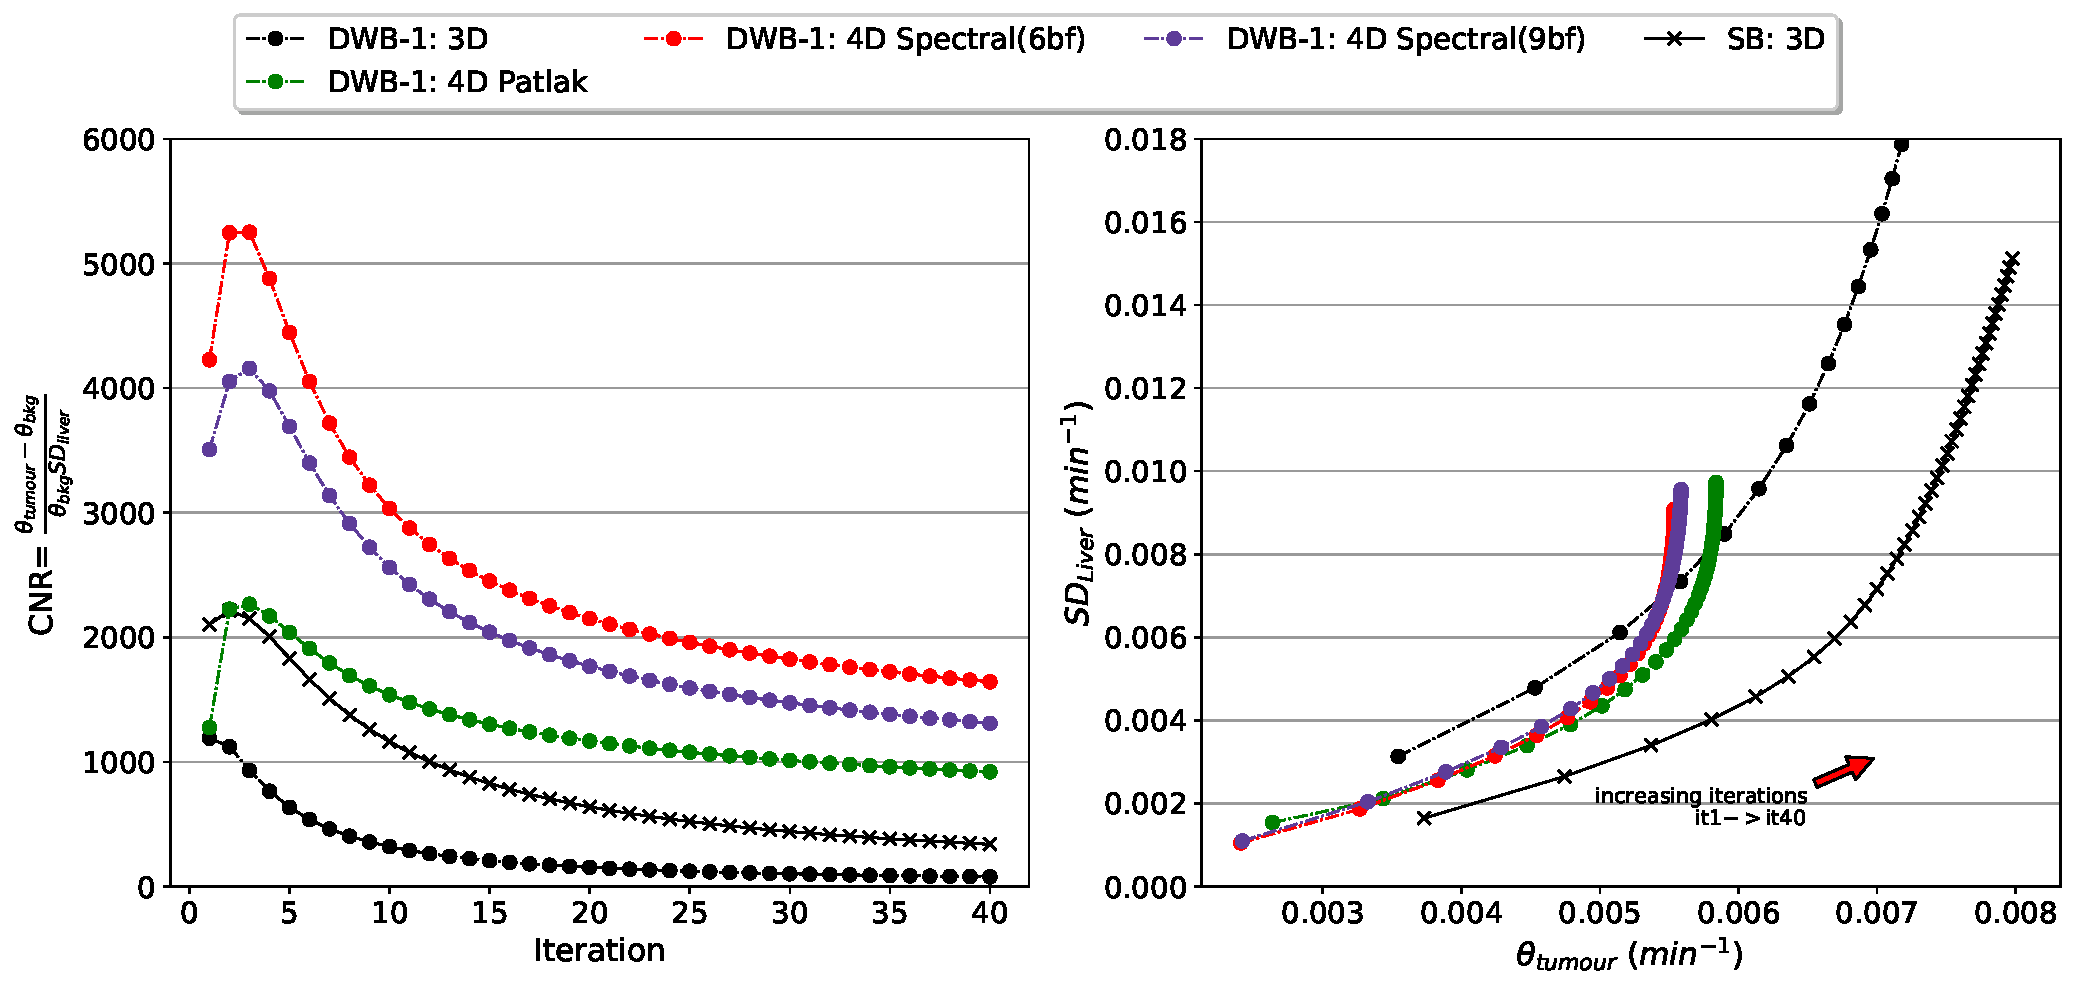
\includegraphics[scale=0.45,angle=0]{./Resume/3_5_tumour_Lung_NoTOF.pdf}
\caption{Données réelles: Rapport contraste/bruit (gauche) et SD du foie par rapport à la moyenne des VOI de la tumeur (droite) pour les reconstructions 3D et 4D.} 
\label{Resumefig:RealData_CNR_CoVBias_NoTOF}
\end{figure} 
%
\begin{figure} [ht!]
\centering
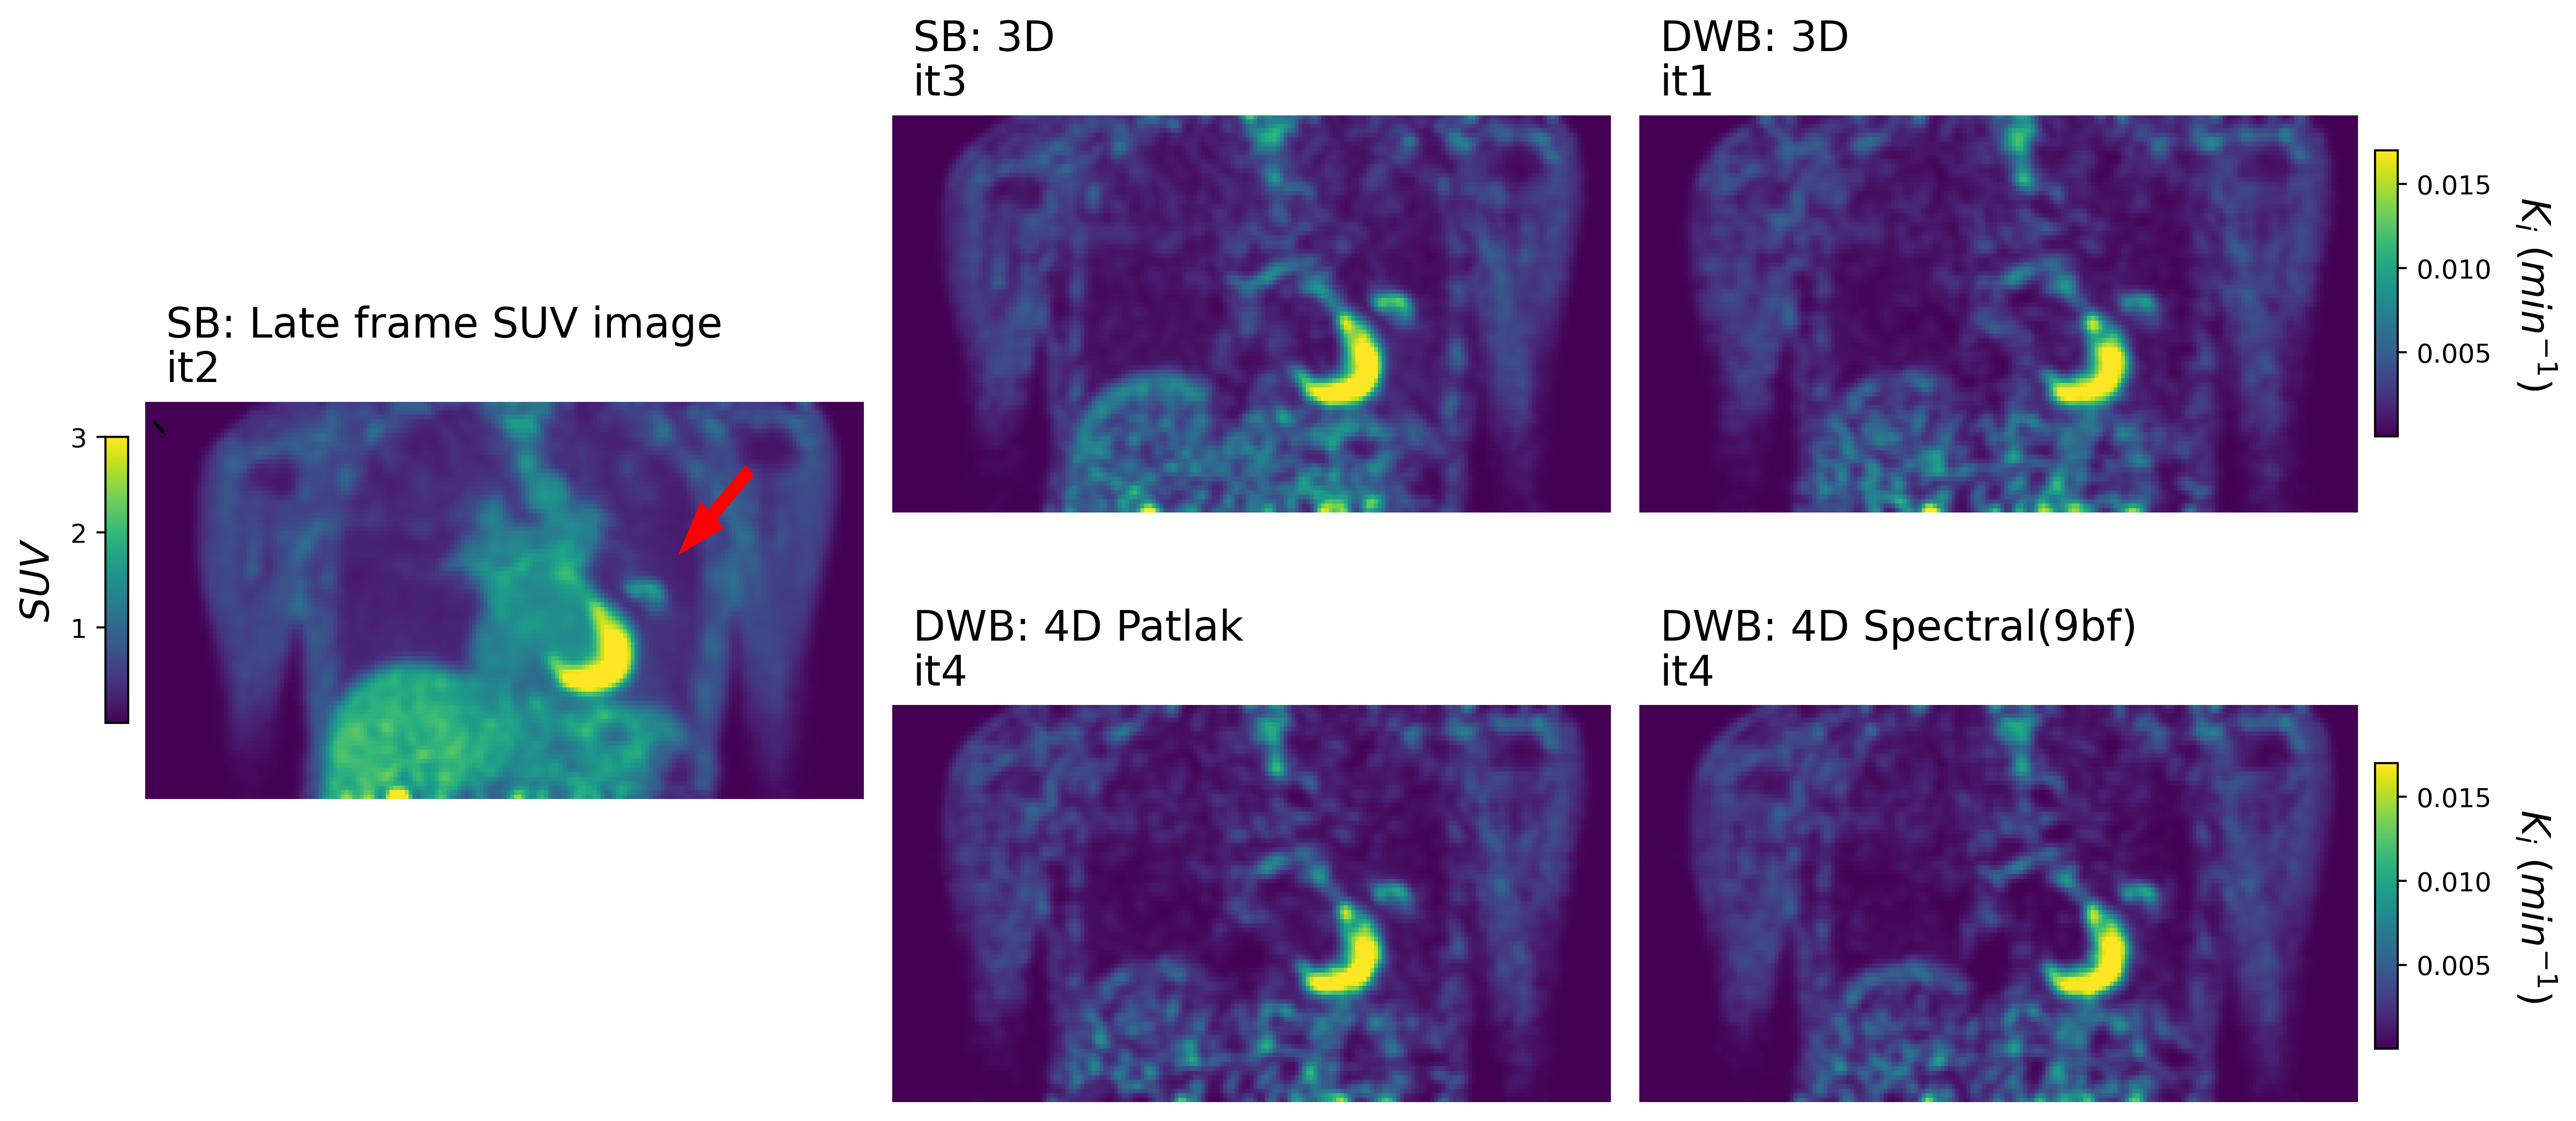
\includegraphics[scale=0.28,angle=0]{./Resume/3_5_RealDataExample.png}
\caption{Données réelles: Les images paramétriques $K_i$ (avec filtrage Gaussien à 5mm) de SB et DWB rejouent des ensembles de données provenant de reconstructions 3D et 4D à des valeurs SD appariées sur le foie.} 
\label{Resumefig:RealKiMontage}
\end{figure} 
%
%
En conclusion, nous avons montré que la reconstruction dynamique 4D est nécessaire en imagerie paramétrique DWB pour obtenir une quantification précise et stable. Pour l'imagerie paramétrique FDG Patlak $K_i$, nous avons montré des résultats de reconstruction dynamique directe Patlak avec des valeurs de bruit et de biais comparables à l'imagerie paramétrique basée sur la reconstruction 3D à partir d'études dynamiques à lit unique. L'utilisation du modèle spectral dans la reconstruction a permis une meilleure utilisation des données dynamiques et une réduction supplémentaire du bruit par rapport à la reconstruction dynamique de Patlak.
Dans l'ensemble, l'utilisation de la reconstruction dynamique 4D pour l'imagerie paramétrique DWB offre des propriétés souhaitables qui permettent la transition de les études dynamiques à lit unique et les pratiques courantes d'imagerie paramétrique par reconstruction 3D sans perte de qualité d'image et avec des avantages supplémentaires pour la précision des images paramétriques. 

\subsection*{Reconstruction dynamique de données DWB: Application d'une étude pharmacocinétique réelle}
Dans ce chapitre, nous décrivons la mise en œuvre des algorithmes de reconstruction dynamique développés précédemment dans un cadre de reconstruction dynamique directe multi-lits au sein de CASToR. Cette approche directe permet d'utiliser toutes les données TEP acquises avec des informations temporelles précises dans une seule boucle de reconstruction, tout en permettant l'utilisation de la reconstruction dynamique directe pour des protocoles d'acquisition DWB plus flexibles et complexes.

Le cadre développé a été appliqué sur des données DWB réelles, qui ont été acquises dans le cadre de l'étude pharmacocinétique IsotoPK~\cite{Marie2019}. 
Le protocole d'acquisition de cette étude commence par une acquisition dynamique à lit unique (Dynamic Single Bed; DSB) de 180 s centrée sur le foie, suivie d'une acquisition DWB de 15 passages WB, pour une durée totale d'une heure. L'étude est réalisée sur des volontaires sains, avec une injection d'un nouveau traceur [$^{11}$C]Glyburide, pour étudier la distribution et la fonction des transporteurs de solutés (SLC) dans la pharmacocinétique des médicaments. Deux scans sont réalisés par volontaire en un seul jour, respectivement sans et avec l'utilisation de l'inhibiteur (rifampicine), appelés scans \textit{CTRL} et \textit{RIF}.
Des reconstructions dynamiques ont été réalisées avec le modèle spectral et ont été évaluées par rapport à une reconstruction 3D régulière utilisant les données de la courbe temps-activité (TAC) sur les volumes d'intérêt (VOI). Enfin, les reconstructions du modèle spectral ont été utilisées pour générer des images paramétriques $K_1$. Comme les estimations de $K_1$ sont sensibles aux informations dynamiques initiales, qui, pour ce protocole, n'étaient disponibles que pour les emplacements couverts par l'acquisition DSB, les images paramétriques $K_1$ générées n'ont été utilisées que pour l'évaluation des VOI couverts par cette seule acquisition. En outre, la correction de la fraction du sang a été ignorée pour l'imagerie de $K_1$ afin d'éviter l'induction d'un bruit excessif par l'application de cette correction au niveau du voxel ; les images paramétriques estimées de $K_1$ de substitution (symbolisées par $K_1^{*}$) sont donc présentées.

Les résultats de l'analyse VOI, donnés dans la figure~\ref{Resumefig_3_3:IsotoPK_CTRL_DWB_4D_vs_3D_Central} pour le scan \textit{CTRL}, ont montré une bonne concordance des TAC entre la reconstruction 3D et spectrale 4D. Les images paramétriques de $K_1^{*}$ issues de la reconstruction spectrale 4D sont présentées dans la figure~\ref{Resumefig_3_3:IsotoPK_K1_SingleSlice} pour les scans du même sujet, avec et sans injection de l'inhibiteur.
%
\begin{figure} [ht!]
\centering
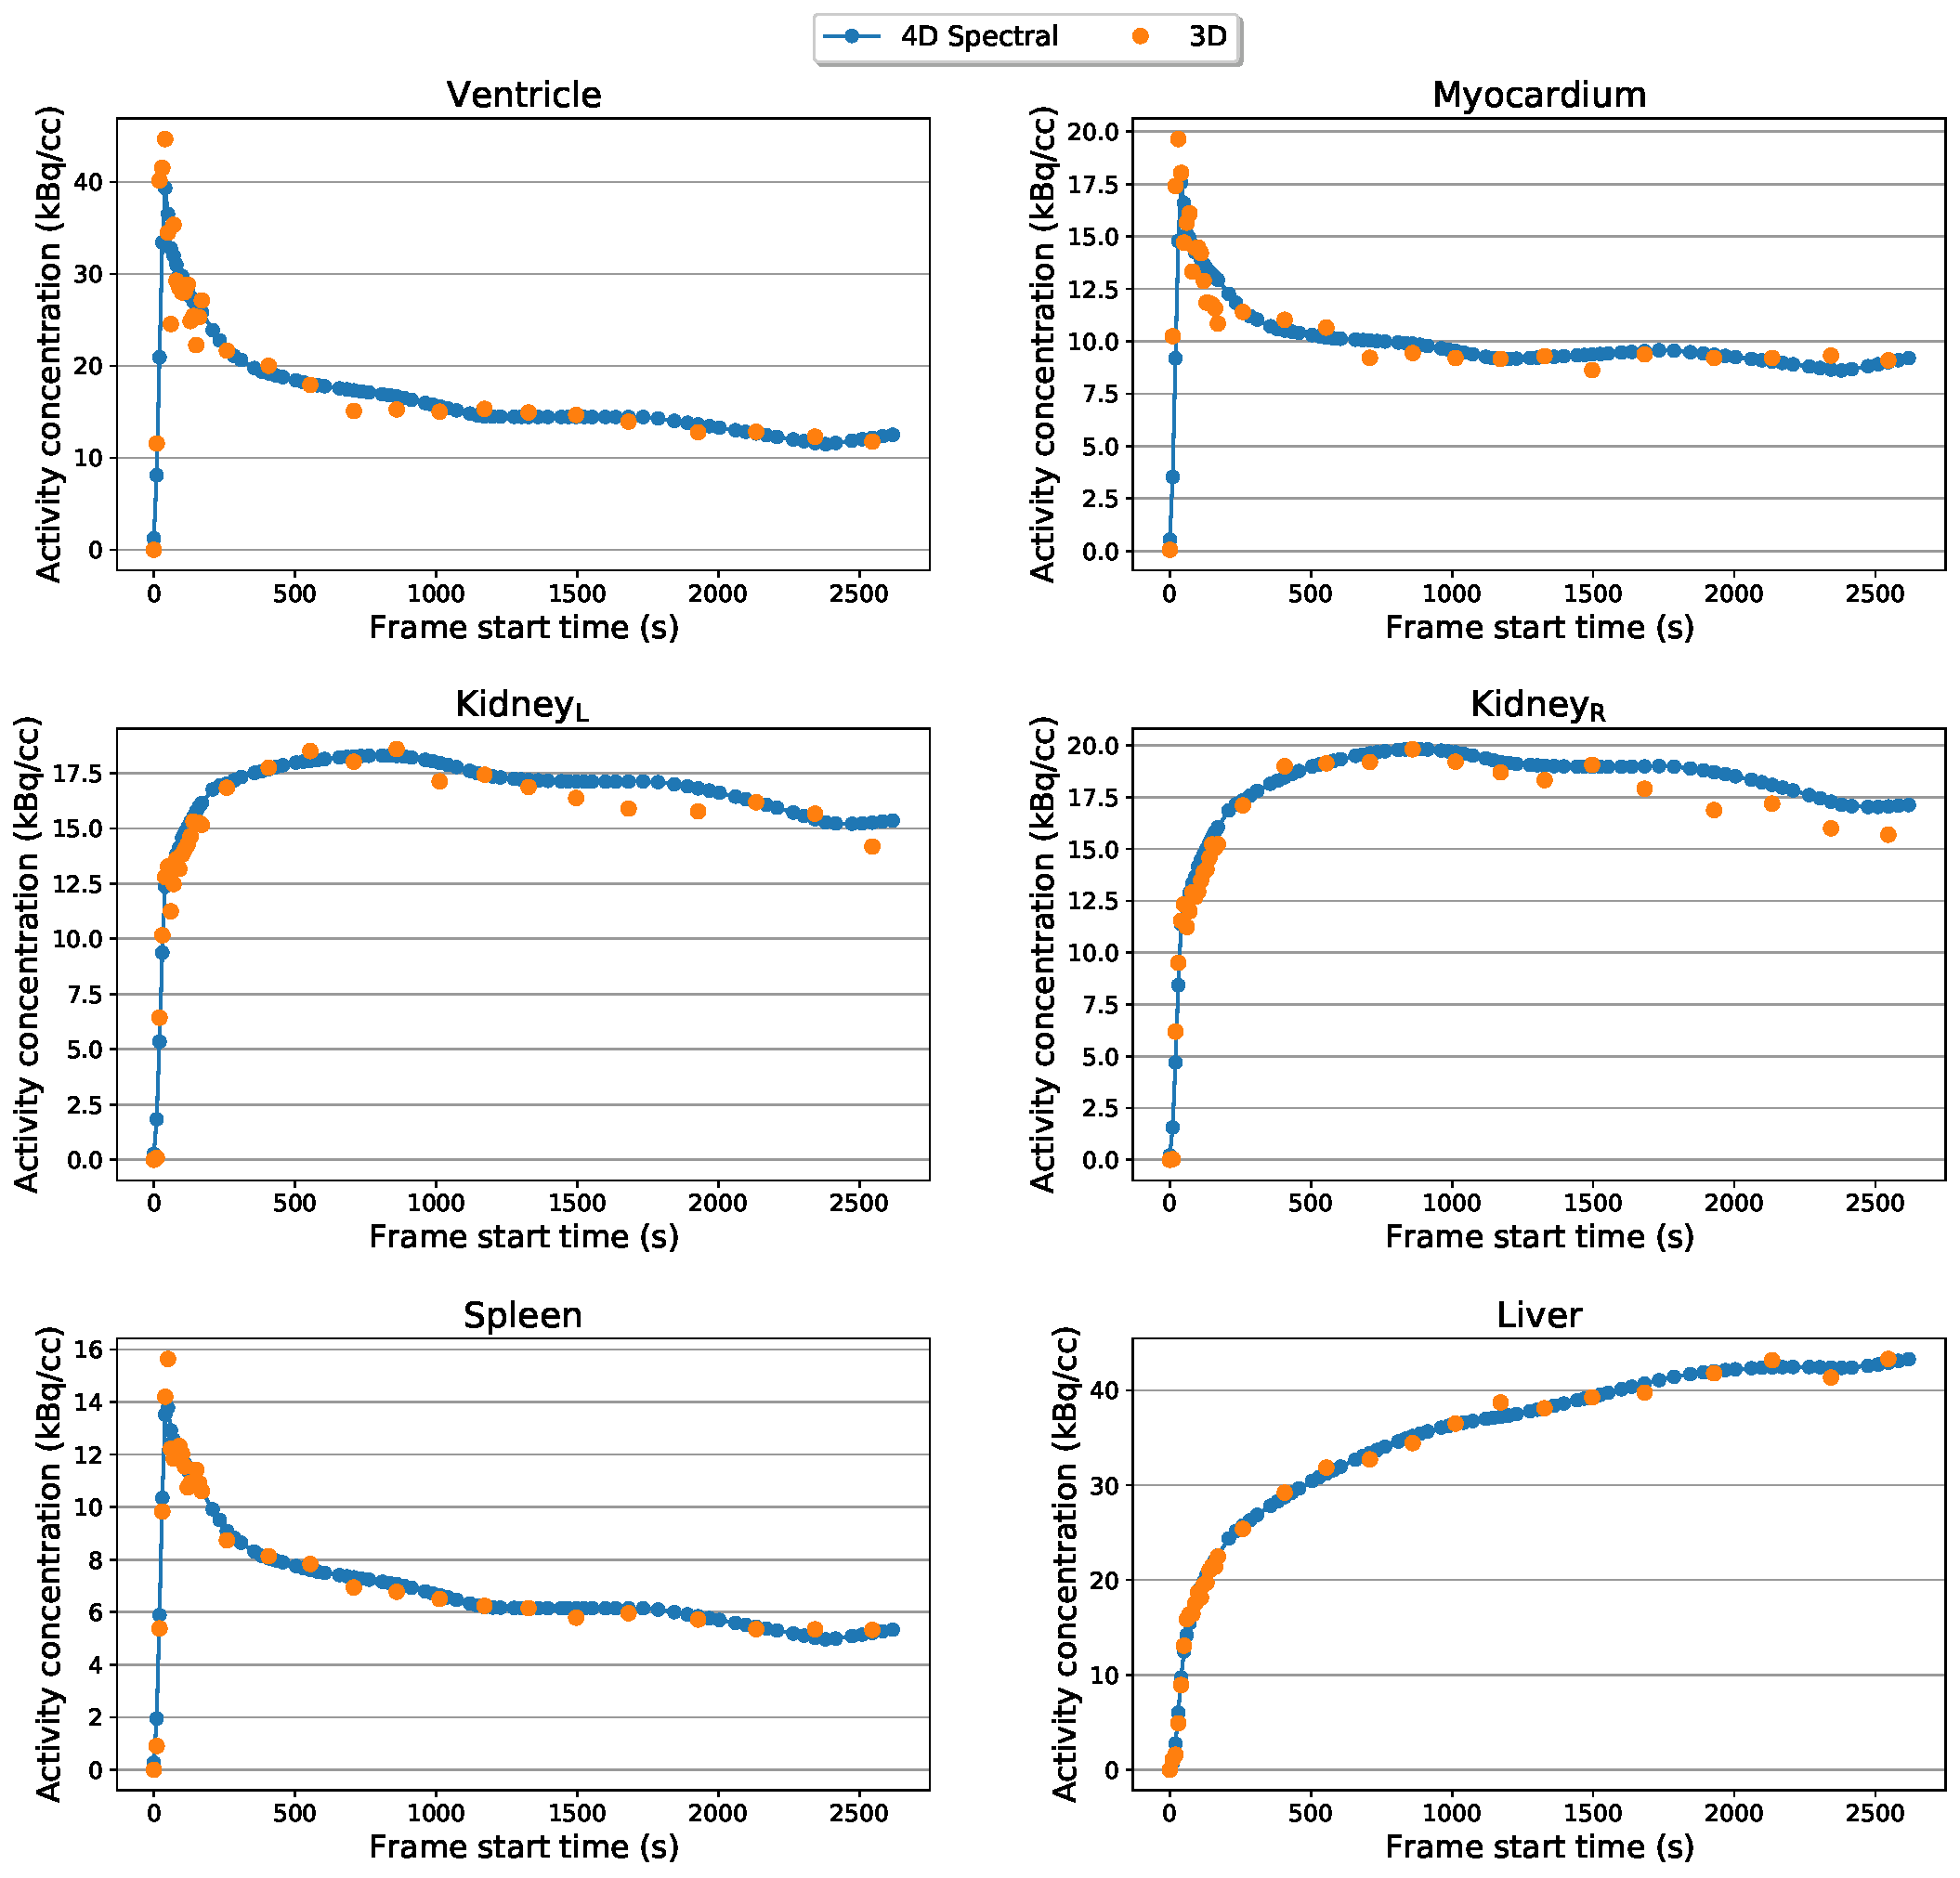
\includegraphics[scale=0.5,angle=0]{./Resume/3_3_IsotoPK_CTRL_DWB_3D_vs_4D_central.pdf}
\caption{Courbes d'activité temporelle moyenne des VOI pour la reconstruction spectrale 3D et 4D. Régions VOI indiquées qui sont incluses dans l'acquisition DSB et DWB.}
\label{Resumefig_3_3:IsotoPK_CTRL_DWB_4D_vs_3D_Central}
\end{figure}
%
\begin{figure} [ht!]
\centering
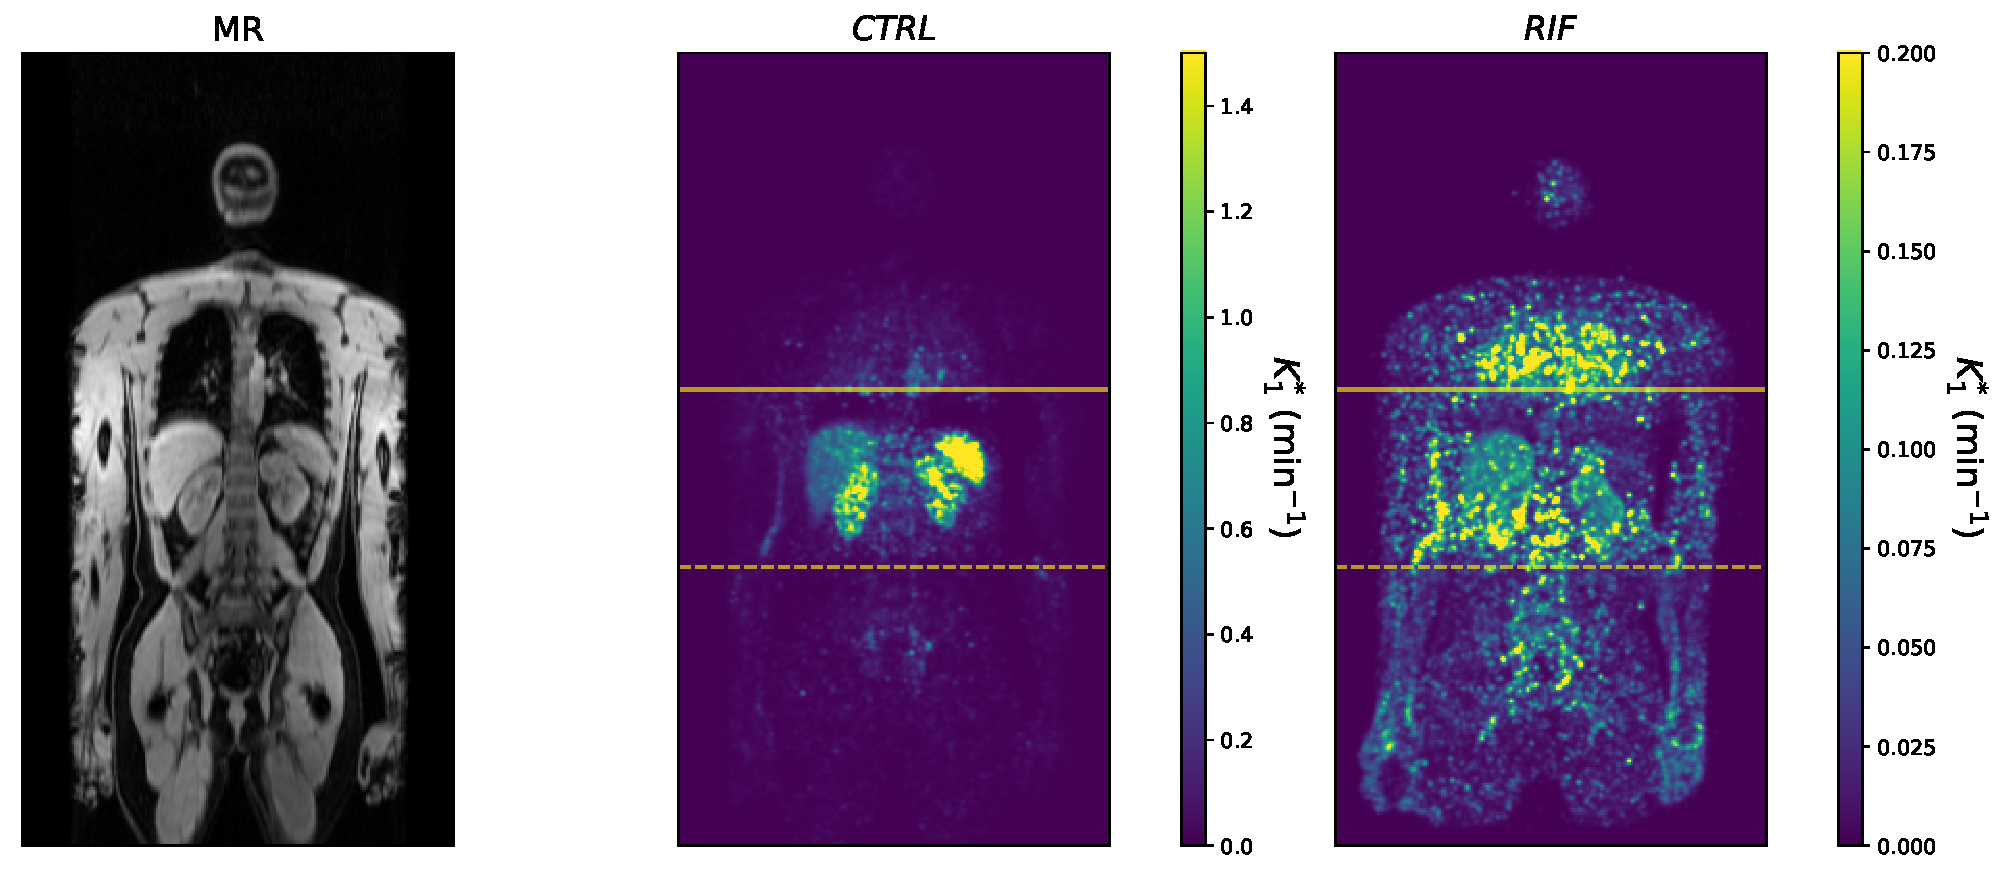
\includegraphics[scale=0.5,angle=0]{./Resume/3_3_IsotoPK_K1_SingleSlice.pdf}
\caption{$K_1$ estimé à partir de la reconstruction spectrale 4D pour les régions VOI incluses dans les acquisitions DSB et DWB, présentées pour les balayages \textit{CTRL} et \textit{RIF}.}
\label{Resumefig_3_3:IsotoPK_K1_SingleSlice}
\end{figure} 
%
En outre, nous présentons dans ce chapitre la mise en œuvre et les résultats des tests d'un algorithme de reconstruction dynamique innovant avec la modélisation résiduelle adaptative pour détecter et corriger toute écart du modèle dynamique. Ces sont particulièrement importantes pour la reconstruction dynamique, car le processus de mise à jour tomographique est lié au modèle dynamique et les erreurs d'ajustement du modèle dynamique peuvent se propager spatialement à d'autres régions. 
Dans l'étude IsotoPK, la principale erreur concernée était le processus de remplissage de la vessie qui était mal modélisé par le modèle spectral.
Nos résultats utilisant la modélisation résiduelle adaptative dans la reconstruction dynamique ont montré des améliorations significatives dans le TAC de la vessie, où l'algorithme adaptatif a réussi à détecter et à corriger le processus de remplissage, au prix d'un bruit d'image supplémentaire sur toutes les régions. Les résultats optimaux ont été obtenus avec une combinaison de filtrage spatial et temporel dans le traitement des données résiduelles avant la modélisation résiduelle, en termes de sélectivité de l'algorithme et de niveaux de bruit ajouté. 

\section*{Conclusions et perspectives}
L'imagerie TEP dynamique sur le corps entier a le potentiel d'augmenter la valeur de l'imagerie TEP, en permettant d'étendre au corps entier l'imagerie TEP et paramétrique entièrement quantitative. 
Dans le processus de transition des études dynamiques à lit unique aux études DWB à lits multiples, il y a une perte considérable de statistiques de données TEP et de fréquence d'échantillonnage. La reconstruction dynamique peut faciliter cette transition en compensant la perte de qualité de l'image et en offrant des avantages supplémentaires pour la précision des images paramétriques. 
Il est possible de réduire davantage le bruit de l'image en optimisant le protocole d'acquisition ou en utilisant des modes d'acquisition améliorés pour l'imagerie DWB, comme la acquisition CBM. 

Nous avons montré avec succès qu'avec l'utilisation du modèle d'analyse spectrale, l'utilisation de toutes les données dynamiques dans une reconstruction unique et l'utilisation de la modélisation résiduelle adaptative, un algorithme générique de reconstruction dynamique peut être appliqué pour pratiquement tous les types d'acquisitions DWB. Cette reconstruction fournit une régularisation temporelle sur les estimations d'activité et permettant la génération de certaines images paramétriques lorsque celles-ci sont pertinentes pour l'étude.

Plusieurs aspects liés à l'estimation des types de mouvements complexes présentés pendant la durée typique d'une étude DWB, que ils doivent être pris en compte dans la reconstruction dynamique pour garantir une imagerie sans erreur et sans artefact.
Récemment, avec le développement de nouveaux scanners à FOV étendu~\cite{Karp2020,Siegel2020} et de scanners corps total~\cite{Cherry2018}, il y a un regain d'intérêt pour résoudre ces problèmes pour l'imagerie dynamique du corps entier. 
Bien que les scanners à A-FOV étendu puissent certainement bénéficier de l'estimation des images paramétriques de la DWB, en particulier celles sensibles à la cinétique rapide précoce après l'injection, leur disponibilité dans les environnements cliniques sera un sujet de préoccupation pendant au moins un certain temps. Les processus dynamiques plus lents peuvent encore être échantillonnés efficacement sur l'ensemble du corps avec les scanners actuels et les protocoles de DWB multi-lits, tels que ceux récemment introduits dans certains scanners commerciaux~\cite{Hu2020}, qui peuvent être plus rentables et plus facilement accessibles dans les environnements cliniques.
Nous nous attendons donc à ce que le regain d'intérêt pour l'imagerie paramétrique du corps entier et l'imagerie quantitative complète se traduise par des avancées qui bénéficieront à l'imagerie DWB pour les scanners de tous les A-FOV et pour différents protocoles d'acquisition. 
